\documentclass{scrartcl}

\usepackage{amssymb}
\usepackage{amsmath}
\usepackage{tikz}
\usetikzlibrary{calc,intersections,through,backgrounds,patterns}
\usetikzlibrary{decorations.text, decorations.markings, fit, arrows, arrows.meta}

\def\centerarc[#1](#2)(#3:#4:#5)% Syntax: [draw options] (center) (initial angle:final angle:radius)
{ \draw[#1] ($(#2)+({#5*cos(#3)},{#5*sin(#3)})$) arc (#3:#4:#5); }

%Chiang & Wainwright - Fundamental Methods of Mathematical Economics (4th Ed.), p. 619, fig 19.3

\begin{document}
	
	%\begin{figure}
	%	\centering
	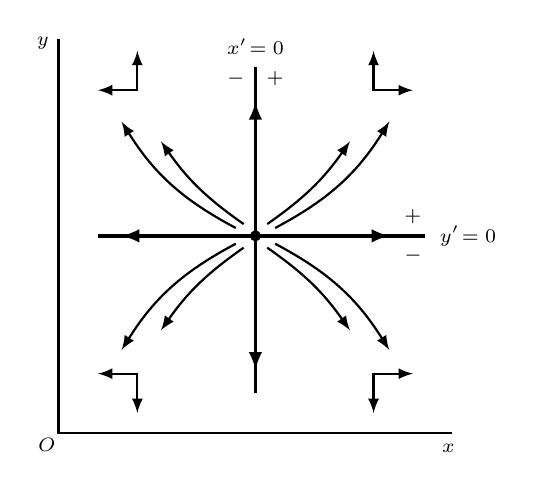
\begin{tikzpicture}
	%axis
	\draw[thick] (-2.5,-2.514)--(-2.5,2.5);	%vertical line
	\draw[thick] (-2.5,-2.5)--(2.5,-2.5);	%horizontal line
		\node at (-2.65,-2.65) {{\scriptsize $O$}};
		\node at (2.45,-2.7) {{\scriptsize $x$}};
		\node at (-2.7,2.45) {{\scriptsize $y$}};
	
	%inner lines
	\fill (0,0) circle (2pt);
	\draw[very thick] (0,-2)--(0,2.15);		%vertical line
	\draw[very thick] (-2,0)--(2.15,0);		%horizontal line
	
	%inner captions
	\node at (0,2.4) {{\scriptsize $x'\!= 0$}};		%NB: reversed in rest
	\node at (2.7,0) {{\scriptsize $y'\!= 0$}};
	%\node at (-0.2,0.2) {{\scriptsize $E$}};				%overlaps small arrow - fix somehow
		\node at (-0.25,2) {{\scriptsize $-$}};	%upper-left
		\node at  (0.25,2) {{\scriptsize $+$}};	%upper-right
		%
		\node at  (2,0.25) {{\scriptsize $+$}};	%right-upper
		\node at (2,-0.25) {{\scriptsize $-$}};	%right-lower
	
	%corner arrows
	\draw[->,>=latex,thick] (-1.5,1.836)--(-1.5,2.35);	%NW: up
	\draw[->,>=latex,thick] (-1.5,1.85)--(-2,1.85);		%NW: left
	%
	\draw[->,>=latex,thick] (1.5,1.836)--(1.5,2.35);	%NE: up
	\draw[->,>=latex,thick] (1.5,1.85)--(2,1.85);		%NE: left
	%
	\draw[->,>=latex,thick] (-1.5,-1.7357)--(-1.5,-2.25);%SW: up
	\draw[->,>=latex,thick] (-1.5,-1.75)--(-2,-1.75);	%SW: left
	%
	\draw[->,>=latex,thick] (1.5,-1.7357)--(1.5,-2.25);	%SE: up
	\draw[->,>=latex,thick] (1.5,-1.75)--(2,-1.75);		%SE: right
	
	%inner arrows
	\draw[->,>=latex,thick] (-0.15,0.15) to[bend left=10] (-1.2,1.2);		%NW - small
		\draw[->,>=latex,thick] (-0.25,0.1) to[bend left=15] (-1.7,1.45);	%NW - big
	%
	\draw[->,>=latex,thick] (0.15,0.15) to[bend right=10] (1.2,1.2);		%NE - small
		\draw[->,>=latex,thick] (0.25,0.1) to[bend right=15] (1.7,1.45);	%NE - big
	%
	\draw[->,>=latex,thick] (-0.15,-0.15) to[bend right=10] (-1.2,-1.2);	%SE - small
	\draw[->,>=latex,thick] (-0.25,-0.1) to[bend right=15] (-1.7,-1.45);	%SE - big
	%
	\draw[->,>=latex,thick] (0.15,-0.15) to[bend left=10] (1.2,-1.2);		%NE - small
	\draw[->,>=latex,thick] (0.25,-0.1) to[bend left=15] (1.7,-1.45);		%NE - big
	
	%for smaller arrows, can also use:
	%\draw[->,>=latex,thick] (-0.15,0.15) to[bend left=10] (-0.75,1);			%NW - small
		%\draw[->,>=latex,thick] (-0.25,0.1) to[bend left=10] (-1.35,1.35);		%NW - big
	
	%arrows on axis
	\draw[->,>=latex,very thick] (0,1.65)--(0,1.7);		%N
	\draw[->,>=latex,very thick] (0,-1.65)--(0,-1.7);	%S
	\draw[->,>=latex,very thick] (-1.65,0)--(-1.7,0);	%E
	\draw[->,>=latex,very thick] (1.65,0)--(1.7,0);		%W
	\end{tikzpicture}
	%	\caption{(a)}
	%\end{figure}
	%
	%
	\hspace{0.75cm}
	%
	%
	%\begin{figure}
	%	\centering
	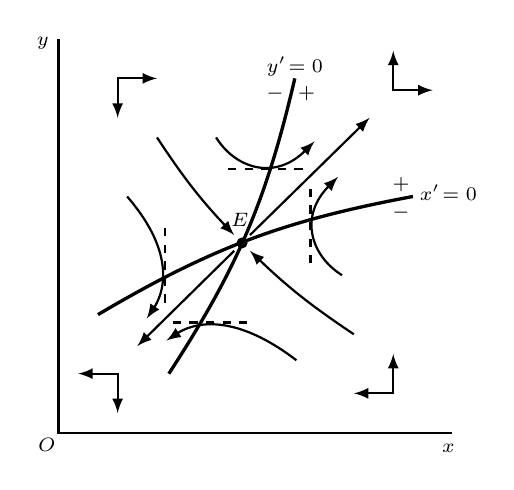
\begin{tikzpicture}
	%axis
	\draw[thick] (-2.5,-2.514)--(-2.5,2.5);	%vertical axis
	\draw[thick] (-2.5,-2.5)--(2.5,-2.5);	%horizontal axis
		\node at (-2.65,-2.65) {{\scriptsize $O$}};
		\node at (2.45,-2.7) {{\scriptsize $x$}};
		\node at (-2.7,2.45) {{\scriptsize $y$}};
	
	%inner lines
	\draw[very thick] (-2,-1) to[bend left=10] (2,0.5);			%x-axis
	\draw[very thick] (-1.1,-1.75) to[bend right=10] (0.5,2);	%y-axis
		\fill (-0.17,-0.09) circle (2pt);
	
	%inner captions
	\node at (0.5,2.15) {{\scriptsize $y'\!= 0$}};
	\node at (2.45,0.55) {{\scriptsize $x'\!= 0$}};
	\node at (-0.2,0.2) {{\scriptsize $E$}};
		\node at (0.25,1.8) {{\scriptsize $-$}};	%upper-left
		\node at (0.65,1.8) {{\scriptsize $+$}};	%upper-right
		%
		\node at (1.85,0.65) {{\scriptsize $+$}};	%right-upper
		\node at (1.85,0.30) {{\scriptsize $-$}};	%right-lower
	
	%inner arrows
	\draw[->,>=latex,thick] (-0.27,-0.19)--(-1.5,-1.4);		%SW
	\draw[->,>=latex,thick] (-0.07,0.01)--(1.45,1.5);		%NE
		%\draw[thick,red] (-1.5,-1.4)--(1.45,1.5);		%test
	\draw[->,>=latex,thick] (-1.25,1.25) to[bend right=5] (-0.27,0.01);		%NW
	\draw[->,>=latex,thick] (1.25,-1.25) to[bend left=5] (-0.07,-0.19);		%SE
	%
	\draw[->,>=latex,thick] (-0.5,1.25) .. controls (-0.25,0.85) and (0.25,0.7) .. (0.75,1.2);	%N
	\draw[->,>=latex,thick] (1.1,-0.5) .. controls (0.7,-0.25) and (0.55,0.25) .. (1.05,0.75);	%E
	\draw[->,>=latex,thick] (-1.63,0.5) .. controls (-0.98,-0.25) and (-1.18,-0.75) .. (-1.38,-1.05);  %W
	\draw[->,>=latex,thick] (0.52,-1.58) .. controls (-0.33,-0.93) and (-0.83,-1.13) .. (-1.13,-1.33);  %S
	
	%dashed lines
	\draw[thick,dashed] (-0.35,0.85)--(0.685,0.85);		%N
	\draw[thick,dashed] (-1.15,-0.85)--(-1.15,0.1);		%W
	\draw[thick,dashed] (-1.05,-1.1)--(0,-1.1);			%S
	\draw[thick,dashed] (0.7,-0.35)--(0.7,0.685);		%E
	
	%corner arrows
	\draw[->,>=latex,thick] (-1.75,2.014)--(-1.75,1.5);		%NW: down
	\draw[->,>=latex,thick] (-1.75,2)--(-1.25,2);			%NW: right
	%
	\draw[->,>=latex,thick] (1.75,1.836)--(1.75,2.35);		%NE: up
	\draw[->,>=latex,thick] (1.75,1.85)--(2.25,1.85);		%NE: left
	%
	\draw[->,>=latex,thick] (-1.75,-1.7357)--(-1.75,-2.25);	%SW: up
	\draw[->,>=latex,thick] (-1.75,-1.75)--(-2.25,-1.75);	%SW: left
	%
	\draw[->,>=latex,thick] (1.75,-2.014)--(1.75,-1.5);		%SE: up
	\draw[->,>=latex,thick] (1.75,-2)--(1.25,-2);			%SE: left
	
	%\draw[help lines] (-2.5,-2.5) grid (2.5,2.5);
	\end{tikzpicture}
	%	\caption{(b)}
	%\end{figure}
	
	
	\vspace{1.25cm}
	
	
	%\begin{figure}
	%	\centering
	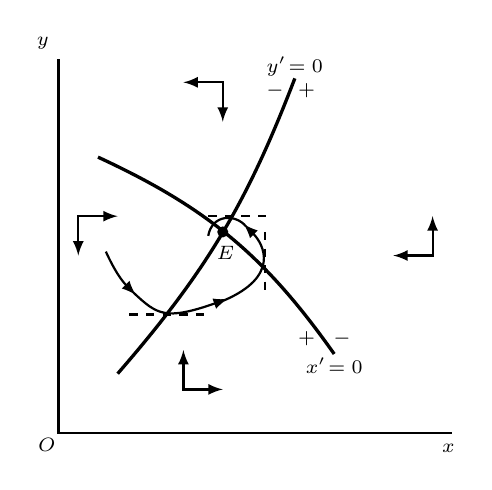
\begin{tikzpicture}
	%axis
	\draw[thick] (-2.5,-2.514)--(-2.5,2.25);	%vertical line
	\draw[thick] (-2.5,-2.5)--(2.5,-2.5);		%horizontal line
		\node at (-2.65,-2.65) {{\scriptsize $O$}};
		\node at (2.45,-2.7) {{\scriptsize $x$}};
		\node at (-2.7,2.45) {{\scriptsize $y$}};
	
	%inner lines
	\draw[very thick] (-2,1) to[bend left=15] (1,-1.5);			%x-axis
	\draw[very thick] (-1.75,-1.75) to[bend right=10] (0.5,2);	%y-axis
		\fill (-0.415,0.05) circle (2pt);
	
	%inner captions
	\node at (0.5,2.15) {{\scriptsize $y'\!= 0$}};
	\node at (1,-1.65) {{\scriptsize $x'\!= 0$}};
	\node at (-0.38,-0.22) {{\scriptsize $E$}};
		\node at (0.25,1.85) {{\scriptsize $-$}};	%upper-left
		\node at (0.65,1.85) {{\scriptsize $+$}};	%upper-right
		%
		\node at (0.65,-1.3) {{\scriptsize $+$}};	%right-upper
		\node at (1.10,-1.3) {{\scriptsize $-$}};	%right-lower
	
	%inner arrows - from outermost to innermost
	%\draw[->,>=latex,thick] (-0.5,1.25) .. controls (-0.25,0.85) and (0.25,0.7) .. (0.75,1.2);
	\draw[->,>=latex,thick] (-1.9,-0.2) to[bend right=10] (-1.52,-0.75);
	\draw[->,>=latex,thick] (-1.55,-0.72) .. controls (-1.25,-1) and (-1.15,-1.08) .. (-0.35,-0.8);
	\draw[->,>=latex,thick] (-0.4,-0.82) .. controls (0.3,-0.52) and (0.12,-0.12) .. (-0.15,0.15);
	\draw[thick] (-0.12,0.12) .. controls (-0.25,0.28) and (-0.55,0.28) .. (-0.6,0);
	
	%dashed lines
	\draw[thick,dashed] (-0.6,0.25)--(0.15,0.25);	%N
	\draw[thick,dashed] (-1.6,-1)--(-0.6,-1);		%S
	\draw[thick,dashed] (0.125,0.05)--(0.125,-0.7);	%E
	
	%corner arrows
	\draw[->,>=latex,thick] (-0.415,1.964)--(-0.415,1.45);		%N: down
	\draw[->,>=latex,thick] (-0.415,1.95)--(-0.915,1.95);		%N: left
	%
	\draw[->,>=latex,thick] (-0.915,-1.9643)--(-0.915,-1.45);	%S: up
	\draw[->,>=latex,thick] (-0.915,-1.95)--(-0.415,-1.95);		%S: right
	%
	\draw[->,>=latex,thick] (-2.25,0.264)--(-2.25,-0.25);	%W: down
	\draw[->,>=latex,thick] (-2.25,0.25)--(-1.75,0.25);		%W: right
	%
	\draw[->,>=latex,thick] (2.25,-0.264)--(2.25,0.25);		%E: up
	\draw[->,>=latex,thick] (2.25,-0.25)--(1.75,-0.25);		%E: left
	
	%\draw[help lines] (-2.5,-2.5) grid (2.5,2.5);
	\end{tikzpicture}
	%	\caption{(c)}
	%\end{figure}
	%
	%
	\hspace{1.3cm}
	%
	%
	%\begin{figure}
	%	\centering
	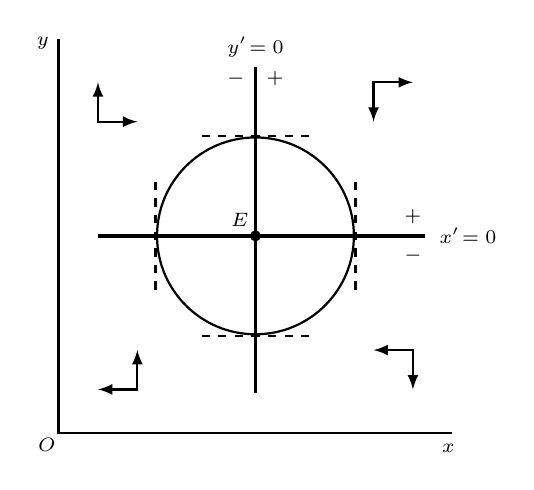
\begin{tikzpicture}
	%axis
	\draw[thick] (-2.5,-2.514)--(-2.5,2.5);	%vertical line
	\draw[thick] (-2.5,-2.5)--(2.5,-2.5);	%horizontal line
		\node at (-2.65,-2.65) {{\scriptsize $O$}};
		\node at (2.45,-2.7) {{\scriptsize $x$}};
		\node at (-2.7,2.45) {{\scriptsize $y$}};
	
		%inner lines
	\fill (0,0) circle (2pt);
	\draw[very thick] (0,-2)--(0,2.15);		%vertical line
	\draw[very thick] (-2,0)--(2.15,0);		%horizontal line
	
	%inner captions
	\node at (0,2.4) {{\scriptsize $y'\!= 0$}};
	\node at (2.7,0) {{\scriptsize $x'\!= 0$}};
	\node at (-0.2,0.2) {{\scriptsize $E$}};				%overlaps small arrow - fix somehow
	\node at (-0.25,2) {{\scriptsize $-$}};	%upper-left
	\node at  (0.25,2) {{\scriptsize $+$}};	%upper-right
	%
	\node at  (2,0.25) {{\scriptsize $+$}};	%right-upper
	\node at (2,-0.25) {{\scriptsize $-$}};	%right-lower
	
	%circle
	\draw[thick] (0,0) circle (1.25cm);
	\draw[thick,dashed] (-0.685,1.27)--(0.685,1.27);		%N
	\draw[thick,dashed] (-1.27,-0.685)--(-1.27,0.685);		%W
	\draw[thick,dashed] (-0.685,-1.27)--(0.685,-1.27);		%S
	\draw[thick,dashed] (1.27,-0.685)--(1.27,0.685);		%E
	
	%arrows on circle
	\centerarc[->,>=latex,thick](0,0)(40:37:1.25)		%NE
	\centerarc[->,>=latex,thick](0,0)(135:132:1.25)		%NW
	\centerarc[->,>=latex,thick](0,0)(220:217:1.25)		%SW
	\centerarc[->,>=latex,thick](0,0)(315:312:1.25)		%SE
	
	%corner arrows
	\draw[->,>=latex,thick] (-2,1.436)--(-2,1.95);		%NW: up
	\draw[->,>=latex,thick] (-2,1.45)--(-1.5,1.45);		%NW: right
	%
	\draw[->,>=latex,thick] (1.5,1.964)--(1.5,1.45);	%NE: down
	\draw[->,>=latex,thick] (1.5,1.95)--(2,1.95);		%NE: right
	%
	\draw[->,>=latex,thick] (-1.5,-1.964)--(-1.5,-1.45);%SE: up
	\draw[->,>=latex,thick] (-1.5,-1.95)--(-2,-1.95);	%SE: left
	%
	\draw[->,>=latex,thick] (2,-1.436)--(2,-1.95);		%SW: down
	\draw[->,>=latex,thick] (2,-1.45)--(1.5,-1.45);		%SW: left
	
	\end{tikzpicture}
	%	\caption{(d)}
	%\end{figure}
	
\end{document}